\documentclass[t,10pt]{beamer}

\mode<presentation>{\usetheme{Goudie}}

\usepackage{amsmath, amsthm, amssymb, mathtools, multirow, dsfont, xcolor, graphicx, lscape, units, tikz, booktabs, fixltx2e, bbm, minted, menukeys}

\usepackage[T1]{fontenc}
\usepackage{lmodern}

% \usepackage[backend=biblatex]{biblatex}%, maxnames=2,firstinits=true,style=apa]{biblatex}
% \bibliography{../../../documents/bib/offline,../../../documents/bib/papers}
% \usepackage[american]{babel}
% \DeclareLanguageMapping{american}{american-apa}

\let\oldfootnote\footnote
\renewcommand\footnote[1][]{\oldfootnote[frame,#1]}

\usetikzlibrary{calc,fit,positioning,shapes,arrows}
\tikzset{>={stealth}}

% symbols
\def\ci{\perp\!\!\!\perp}
\def\notci{\perp\!\!\!\perp\!\!\!\!\!\!\!\!\!\!\;\diagup\;}

% code background
\setminted{bgcolor={lightgraybg}}

\newenvironment{highlightblock}[0]%
  {\begin{beamercolorbox}[sep=1em]{postit}}%
  {\end{beamercolorbox}}

\begin{document}

\title{Simple parallelisation on hpc}
\author{R.J.B. Goudie}
\date{\today}
\maketitle

\begin{frame}{But R is R is R...?!}

\begin{highlightblock}
R code that runs on your desktop/laptop will (almost) always run on the HPC just fine without \textit{any} changes to the R code whatsoever.
\end{highlightblock}

\bigskip
This talk is about using the \textbf{standard R code} you already have, but running it lots of times efficiently, for example for

\begin{itemize}
\item Simulation studies
\item Multiple-chain MCMC
\item GWAS-type problems
\item etc...
\end{itemize}

i.e.\ doing \textit{almost} the same thing lots of times, but rather than doing one after the other, doing all of them simultaneously.

\bigskip
\alert{Each task must be completely independent}
\end{frame}

\begin{frame}[fragile]{Notation and caveats}

\begin{enumerate}
\item Everywhere where you see \mintinline{sh}{abc123} in this talk, replace
with your Cambridge CRSID (Raven) username.

\item When I refer to a file as \mintinline{sh}{~/.ssh/config} this means the file \mintinline{sh}{/home/abc123/.ssh/config} i.e. a file called \mintinline{sh}{config} in the \mintinline{sh}{.ssh} folder in your home folder.


\item node = a single one of the many computers that make up the overall HPC, each of which has a processor on it
\item core = a processor has multiple `cores', each of which can be doing something different
\item Slurm = software that controls the order that jobs are run on the HPC
\end{enumerate}

\bigskip
\textit{Caveat: I use the HPC from my Mac, and use the command line. I might have made mistakes about the situation if your desktop is Linux or Windows.}

\end{frame}

\begin{frame}[fragile]{Faff 1: SecurID}

If you are not using \alert{your BSU desktop} you won't be able to log in directly. You have to log in first using your RSA SecurID token.

\begin{itemize}
\item Use \alert{F5}. Go to \url{https://bsulogin.mrc-bsu.cam.ac.uk}, enter your username and token security number, then click ``Netowrk access MRC BSU'' button. Install the plugin if requested.

\bigskip

\includegraphics[width=0.2\textwidth]{f5-screen1.png}
\hspace{1em}

\includegraphics[width=0.235\textwidth]{f5-screen2.png}
\bigskip

\item On iOS (iPad and iPhone), download \alert{F5 BIG-IP Edge Client}\footnote{\url{https://itunes.apple.com/app/id411062210}}

\item You can also use \alert{SSH Tunnelling}, which is a little more faff to set up.
\end{itemize}

\end{frame}


\begin{frame}[fragile]{Faff 2: remembering/typing the tediously long command to log in}

On \alert{Linux/Mac}, the usual way to log in is

\begin{minted}{sh}
ssh abc123@login-mrc-bsu.hpc.cam.ac.uk
\end{minted}

Instead (from a Linux/Mac), add the following to the bottom of (or create new file) \mintinline{sh}{~/.ssh/config}

\begin{minted}{sh}
Host hpc
  User abc123
  HostName login-mrc-bsu.hpc.cam.ac.uk
\end{minted}

Now to log in, just type

\begin{minted}{sh}
ssh hpc
\end{minted}

On \alert{Windows}, use PuTTY\footnote{\url{http://www.chiark.greenend.org.uk/~sgtatham/putty}}
\end{frame}

\begin{frame}[fragile]{Faff 3: having to type your Raven password incessantly}

Set up \alert{passwordless SSH} on Mac/Linux:
\begin{enumerate}
\item Check for an existing ``ssh key'' by checking for a file called \mintinline{sh}{id_rsa.pub}, \mintinline{sh}{id_dsa.pub} or similar in \mintinline{sh}{~/.ssh/} by running \mintinline{sh}{ls -la ~/.ssh/}. If so, skip step 2, \& replace \mintinline{sh}{id_rsa} in step 2+3 with your key's name).

\item Generate a key, and create a ``passphrase'' for the key
\begin{minted}{sh}
ssh-keygen -t rsa -b 4096
\end{minted}

\item Copy the ``public key'' to the HPC
\begin{minted}{sh}
ssh-copy-id -i ~/.ssh/id_rsa.pub abc123@hpc
\end{minted}

\item Setup an ``ssh agent'' to avoid typing the passphrase.
\begin{minted}{sh}
eval "$(ssh-agent -s)"
ssh-add ~/.ssh/id_rsa
\end{minted}
\end{enumerate}

\end{frame}

\begin{frame}[fragile]{Faff 3: continued}

On macOS Sierra\footnote{\url{http://apple.stackexchange.com/a/254714}}, also need to add to your \mintinline{sh}{~/.ssh/config} the following:

\begin{minted}{sh}
Host *
   UseKeychain yes
   AddKeysToAgent yes
\end{minted}

\end{frame}

\begin{frame}[fragile]{Faff 4: your internet connection dies, and you lose what you were doing}

\begin{itemize}
\item Get SSH to say `hello' from time-to-time. Add the following lines to \mintinline{sh}{~/.ssh/config} on your desktop/laptop

\begin{minted}{sh}
ServerAliveInterval 10
ServerAliveCountMax 200
\end{minted}

\item Use GNU \mintinline{sh}{screen}\footnote{\url{https://www.gnu.org/software/screen/}} or \mintinline{sh}{tmux}\footnote{\url{https://tmux.github.io}}.
For screen, when you log in type
\begin{minted}{sh}
screen
\end{minted}

This starts a new `session'. Now if your connection dies, you just log back in with \mintinline{sh}{ssh hpc}, then type \mintinline{sh}{screen -r} and whatever you had open etc is exactly as you left it.
\end{itemize}
\end{frame}

\begin{frame}{Structure of the HPC}

\centering
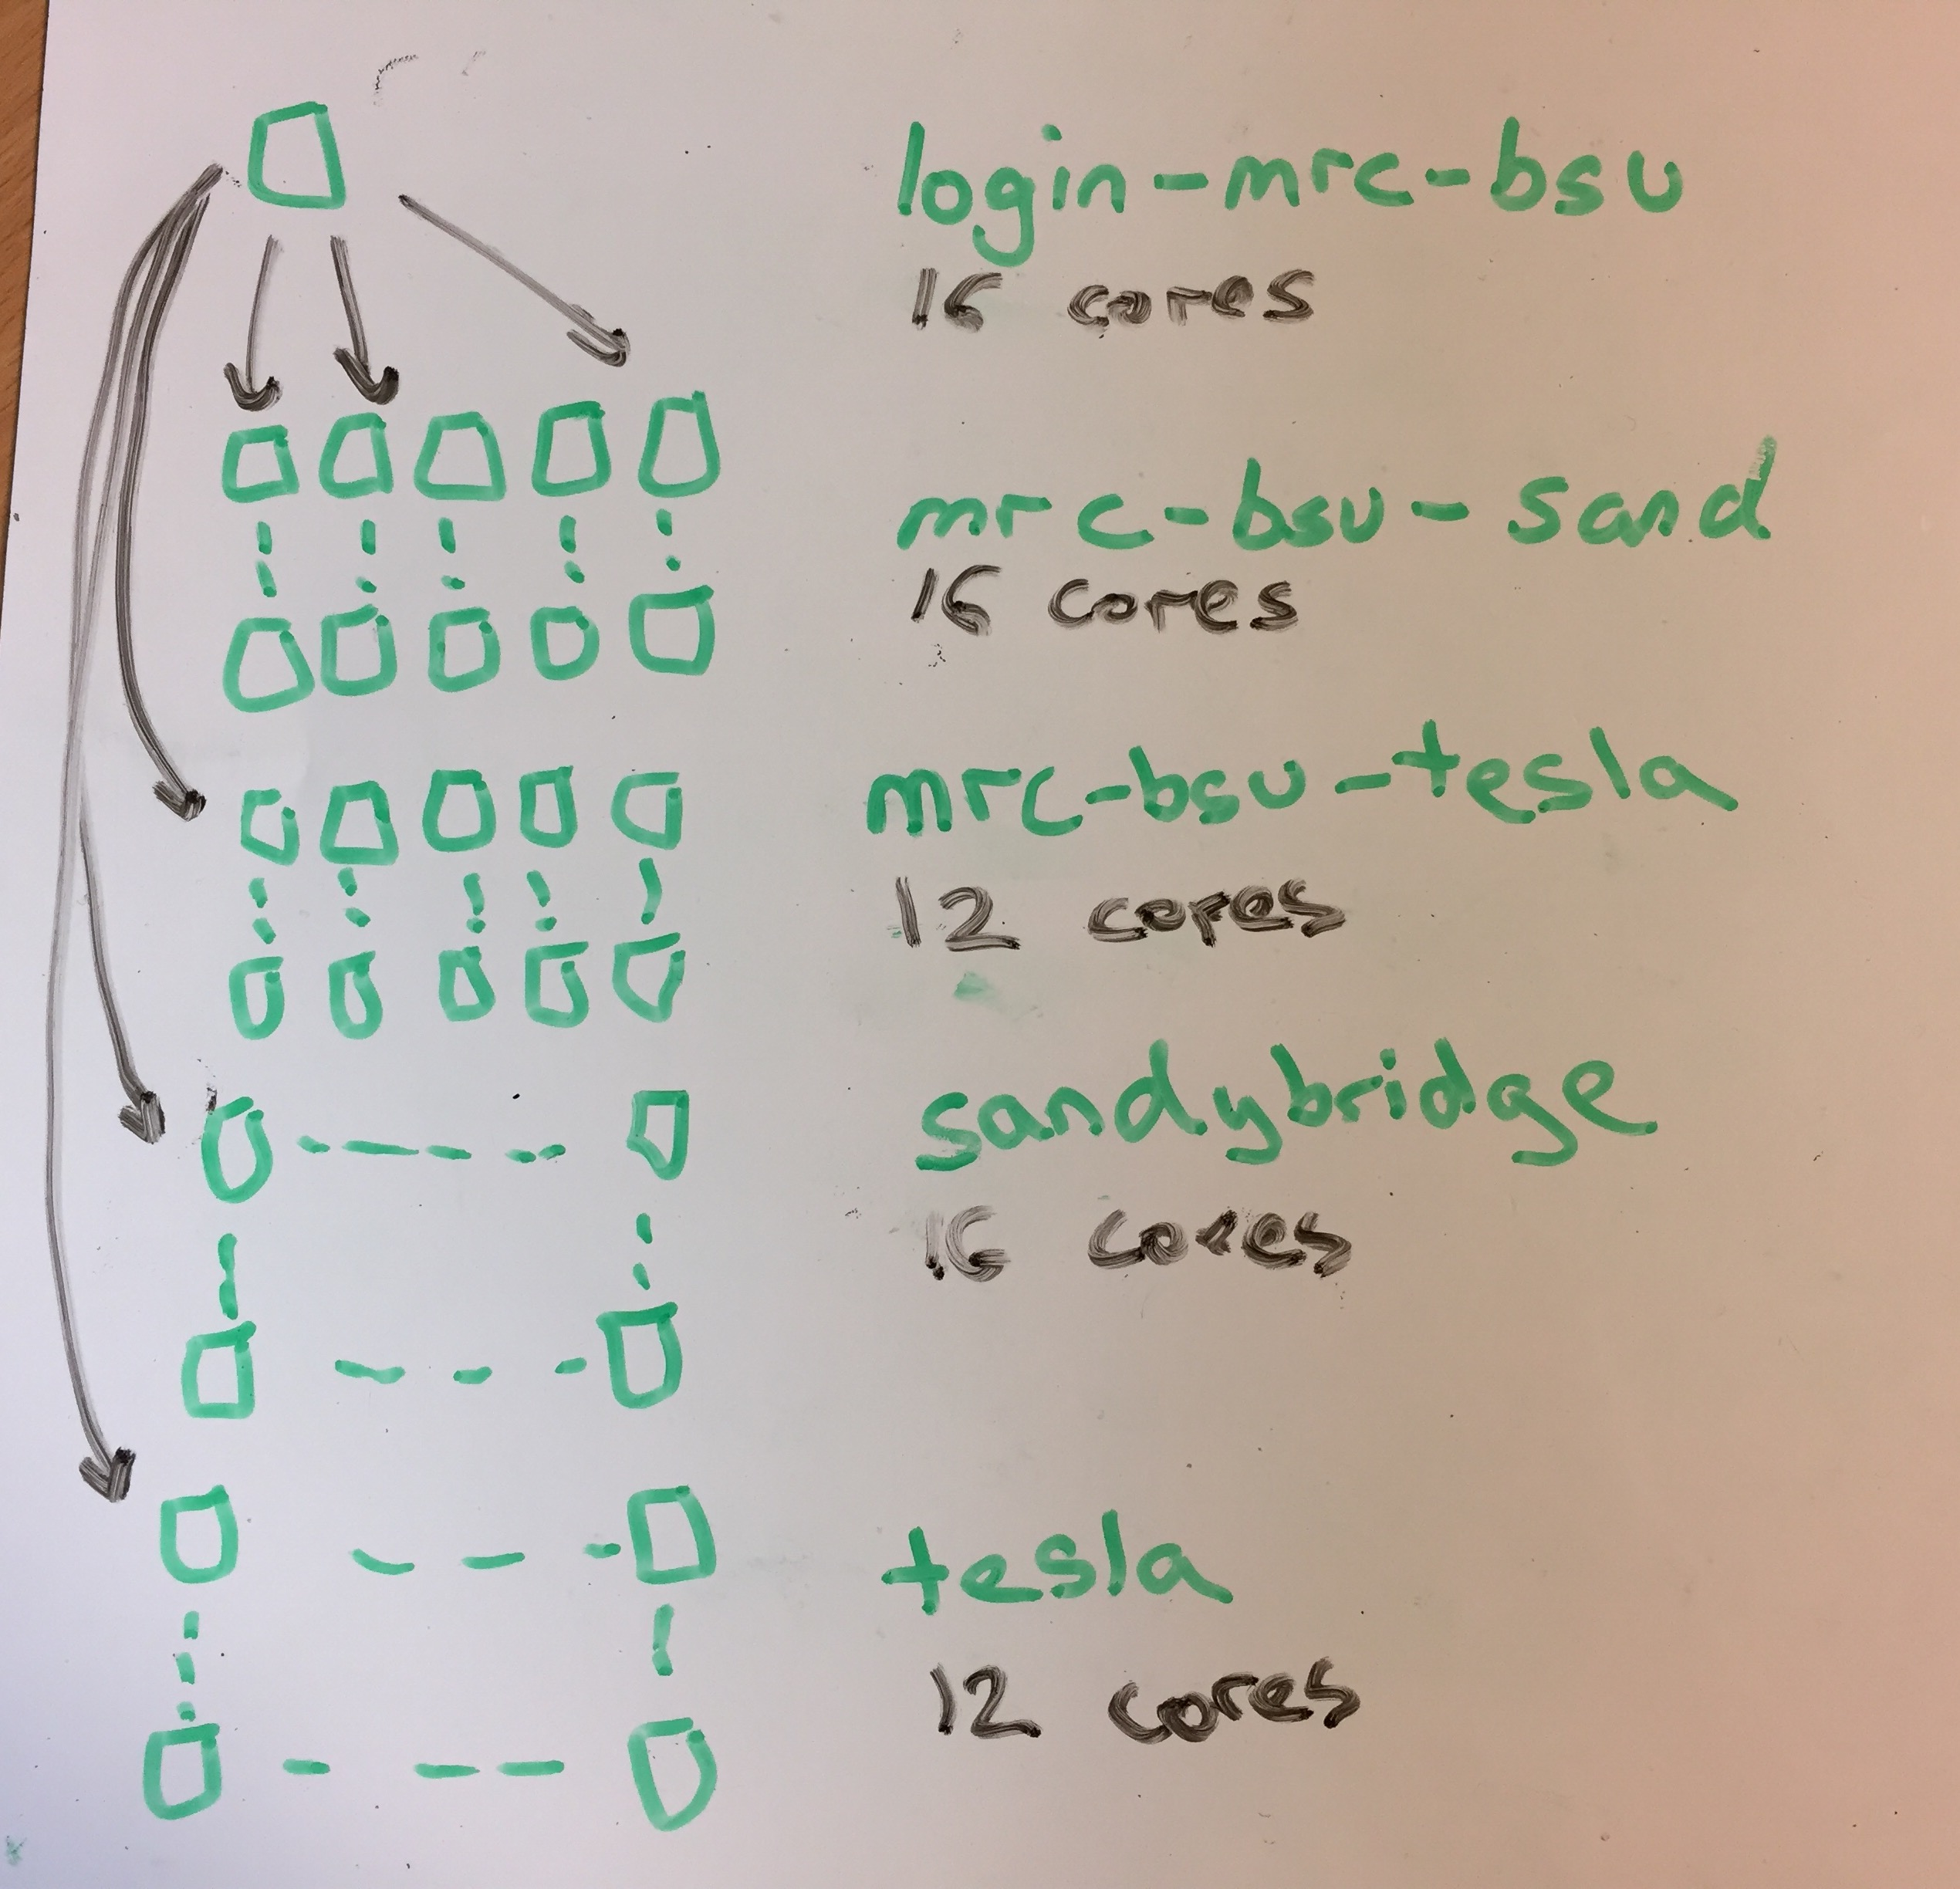
\includegraphics[width=0.8\textwidth]{hpc-structure2}
\end{frame}

\begin{frame}[fragile]{Faff 5: load `modules'}

By default, when you log on to the HPC, \mintinline{sh}{R} is \alert{not available}.

\bigskip
You have to load it using \mintinline{sh}{module}\footnote{\url{http://modules.sourceforge.net}} by typing

\begin{minted}{sh}
module add R/3.3.2
\end{minted}

You can view all the software that is available by typing \mintinline{sh}{module avail}.

\bigskip
To avoid having to type this all the time, add the above to the bottom of \mintinline{sh}{~/.bashrc}, e.g.

\begin{minted}{sh}
module add R
module add htop
\end{minted}
\end{frame}

\begin{frame}[fragile]{Faff 6: having to use the command line}

You can \alert{partly} avoid this.

\begin{itemize}
\item
You can also use \alert{VNC}, see instructions\footnote{\url{http://www.hpc.cam.ac.uk/using-clusters/remote-desktops-and-3d/darwin-turbovnc}}

\item Or (maybe slower?) change \mintinline{sh}{~/.ssh/config} on your Linux/Mac to

\begin{minted}{sh}
Host hpc
  User abc123
  HostName login-mrc-bsu.hpc.cam.ac.uk
  ForwardX11 yes
\end{minted}

Then once you have logged into the HPC type, for example,
\begin{minted}{sh}
module add rstudio
rstudio
\end{minted}
\end{itemize}

\alert{Do not log in as above, start R, and run intensive calculations -- see next slide}

\end{frame}

\begin{frame}[fragile]{login-mrc-bsu, also called the `frontend node'}

This computer \mintinline{sh}{login-mrc-bsu} is what you are using after typing \mintinline{sh}{ssh hpc}

\bigskip
\begin{highlightblock}
Please don't do anything even vaguely intensive on login-mrc-bsu.
\end{highlightblock}

\begin{itemize}
\item Don't start \mintinline{sh}{R} or \mintinline{sh}{rstudio} and run your simulation directly like you would on your desktop, unless it is very quick + simple + low memory.
\item Even people reading in enormous data/results files or \mintinline{sh}{zip}ping enormous files causes problems from time to time.
\end{itemize}

\vspace{\baselineskip}
\alert{Instead: use an `interactive session'. This is really easy to do}. Just type:

\begin{minted}{sh}
sintr -A MRC-BSU-SL2 -p mrc-bsu-sand -N1 -t 1:00:00
\end{minted}
This is then (for 1 hour) your own core on a machine, and you can do whatever you want: including running R, rstudio, zipping 1TB files, ....
\end{frame}

\begin{frame}{How the `queue' works}

Roughly \alert{first come, first served} queue (but not quite).

\bigskip
\begin{itemize}
\item `Fairness' is only considered when a slot is available.
\item You never get kicked off until your time is up, even if you are using the whole cluster and have been for hours.
\end{itemize}

\bigskip
\begin{highlightblock}
Please don't submit jobs that use 100s of cores for hours, except if you use `rate limiting'.
\end{highlightblock}

\end{frame}


\begin{frame}[fragile]{Batch jobs}

Two example batch scripts are put in your filespace on the HPC, but they include a line \mintinline{sh}{Do not change}... which \alert{does need to be changed} for the mrc-bsu cluster...

\bigskip
Instead, you might find my BSU-specific examples useful:

\bigskip
\begin{centering}
\url{https://github.com/rjbgoudie/bsu-cluster}
\end{centering}

\end{frame}

\begin{frame}[fragile]{Running basic 1 core R script}

To run a R script called \mintinline{sh}{myrfile.R} for 1 hour on 1 core:

\begin{enumerate}
\item Download  a submission script, e.g.\footnote{\url{https://github.com/rjbgoudie/bsu-cluster/blob/master/submission-scripts/r-single-core/slurm_submit.mrc-bsu-sand}} by clicking `Raw' then saving the file.

\item Copy \mintinline{sh}{myrfile.R} and \mintinline{sh}{slurm_submit.mrc-bsu-sand} to the HPC.

Easiest to use a SFTP program: e.g.\ Filezilla\footnote{\url{https://filezilla-project.org}}, or lots of other choices for Mac\footnote{\url{http://apple.stackexchange.com/a/25667}} and Linux\footnote{\url{http://askubuntu.com/a/109020}}; WinSCP\footnote{\url{https://winscp.net/}} on Windows.

Connect to \mintinline{text}{login-mrc-bsu.hpc.cam.ac.uk} with username \mintinline{text}{abc123}

\item Log on with \mintinline{sh}{ssh hpc} in a command line window.

\item Submit it:
\begin{minted}{sh}
sbatch slurm_submit.mrc-bsu-sand myrfile.R
\end{minted}
\end{enumerate}
\end{frame}

\begin{frame}[fragile]{Array jobs}

\alert{Running the same R file 1000 times is easy}: download example\footnote{\url{https://github.com/rjbgoudie/bsu-cluster/blob/master/submission-scripts/r-single-core-array/slurm_submit.mrc-bsu-sand}}, or just add the following to submission script (after e.g.\ the \mintinline{text}{#SBATCH --ntasks=1} line)

\begin{minted}{text}
#SBATCH --array=1-1000%50
\end{minted}

The \mintinline{text}{%50} bit means at most 50 tasks will run simultaneously. This `rate limiting' helps smooth about the peaks and troughs in demand.

R can find out which of the 1000 tasks it is processing by

\begin{minted}{r}
task_id_string <- Sys.getenv("SLURM_ARRAY_TASK_ID")
task_id <- as.numeric(task_id_string)

seed <- c(425, 3453, ......., 223, 232)[task_id]
set.seed(seed)
rnorm(100)
\end{minted}

\end{frame}

\begin{frame}[fragile]{Array jobs admin}

Remember to add \mintinline{r}{task_id} to the filenames of all your output, otherwise they will overwrite each other. For example,

\begin{minted}{r}
filename <- paste0("samples_", task_id, ".rds")
saveRDS(samples, file = filename)
\end{minted}

\end{frame}

\begin{frame}[fragile]{Monitoring progress}

To see the status of your jobs
\begin{minted}{sh}
squeue --user=abc123
\end{minted}

If you want this to update `live', use \mintinline{sh}{watch}\footnote{See \url{http://www.linfo.org/watch.html} or \url{https://linux.die.net/man/1/watch}}
\begin{minted}{sh}
watch squeue --user=abc123
\end{minted}

To see a summary of how much of our cluster is being used currently
\begin{minted}{sh}
sinfo --partition=mrc-bsu-sand,mrc-bsu-tesla --format="%P %C"
\end{minted}
I wrote a (trivial) script that presents this marginally more clearly\footnote{\url{https://github.com/rjbgoudie/bsu-cluster/blob/master/bin/bsu-queue-status}}
\end{frame}

\begin{frame}[fragile]{Switching to the bigger University HPC (Darwin/Wilkes)}

BSU have 200,000 (?) free hours on Darwin and Wilkes, and anyway Ela tells me money not an issue.

\bigskip
It is very easy to switch, so please do if you are doing something enormous

\bigskip
All you have to do is change \alert{2 lines} in your submission script.

\bigskip
For standard nodes (`Darwin'/`sandybridge'), change

1. \mintinline{text}{#SBATCH -A MRC-BSU-SL2} to
\mintinline{text}{#SBATCH -A MRC-BSU-SL3}

2. \mintinline{text}{#SBATCH -p mrc-bsu-sand} to \mintinline{text}{#SBATCH -p sandybridge}

\bigskip
For nodes with GPUs (`Wilkes'/`tesla'), change:

1. \mintinline{text}{#SBATCH -A MRC-BSU-SL2-GPU} to
\mintinline{text}{#SBATCH -A MRC-BSU-SL3-GPU}

2. \mintinline{text}{#SBATCH -p mrc-bsu-tesla} to \mintinline{text}{#SBATCH -p tesla}

\bigskip
Everything else is identical.
\end{frame}

\begin{frame}[fragile]{Automating more}

\begin{itemize}
\item Chris Wallace has some Ruby scripts\footnote{\url{https://github.com/chr1swallace/slurmer}}

\item There is an R-package called \mintinline{text}{rslurm}\footnote{\url{https://cran.r-project.org/package=rslurm}}, but I've never used it.

\item I use my own (completely undocumented) R-package \mintinline{r}{mngr}\footnote{\url{https://github.com/rjbgoudie/mngr}}, which automates running `workflows' of R files; using \verb|git| to make jobs reproducible; handling multiple \verb|git| branches; shortcuts for dull admin of filing logs etc.
\end{itemize}

\end{frame}

\begin{frame}{Further help}

\begin{itemize}
\item The university's documentation\footnote{\url{http://www.hpc.cam.ac.uk/using-clusters}} for the university-wide HPC, which is basically identical to the BSU cluster.

\item For technical documentation, use, for example, \mintinline{sh}{man sbatch} on the command-line. Note the HPC uses Slurm version 14.11.8, which is a couple of years old, so the Slurm web documentation\footnote{\url{https://slurm.schedmd.com/man_index.html}} for version 17.02 is occasionally misleading.
\end{itemize}

\end{frame}
\end{document}
